% Source: graduate-coursework/Research/Intro_to_Agents/handouts/Part7_Parallelization.tex

\documentclass[border=4pt]{standalone}
\usepackage{amsmath,amssymb,amsfonts}
\usepackage[T1]{fontenc}
\usepackage{graphicx}
\usepackage{lmodern}
\usepackage{tikz}
\usepackage{xcolor}
\usetikzlibrary{shapes.geometric, arrows.meta, positioning, calc, fit, backgrounds, matrix, decorations.pathreplacing}

\definecolor{UofSCGarnet}{HTML}{73000a}
\definecolor{UofSCBlack}{HTML}{000000}
\definecolor{UofSCWhite}{HTML}{ffffff}
\definecolor{UofSCRose}{HTML}{CC2E40}
\definecolor{UofSCAtlantic}{HTML}{466A9F}
\definecolor{UofSCCongaree}{HTML}{1F414D}
\definecolor{UofSCHorseshoe}{HTML}{65780B}
\definecolor{UofSCGrass}{HTML}{CED318}
\definecolor{UofSCHoneycomb}{HTML}{A49137}
\definecolor{UofSC90Black}{HTML}{363636}
\definecolor{UofSC70Black}{HTML}{5C5C5C}
\definecolor{UofSC50Black}{HTML}{A2A2A2}
\definecolor{UofSCWarmGrey}{HTML}{676156}
\definecolor{UofSCSandstorm}{HTML}{FFF2E3}
\definecolor{UofSCDarkGarnet}{HTML}{570008}
\definecolor{UofSCAzalea}{HTML}{844247}

\tikzset{
    % Node styles - all with sharp corners
    agentbox/.style={
        rectangle,
        draw=UofSCGarnet,
        fill=UofSCSandstorm,
        thick,
        minimum width=2cm,
        minimum height=0.8cm,
        text centered,
        font=\footnotesize
    },
    processbox/.style={
        rectangle,
        draw=UofSCAtlantic,
        fill=UofSCWhite,
        thick,
        minimum width=2.5cm,
        minimum height=0.7cm,
        text centered,
        font=\footnotesize
    },
    syncbox/.style={
        rectangle,
        draw=UofSCCongaree,
        fill=UofSCCongaree!20,
        thick,
        minimum width=3cm,
        minimum height=0.5cm,
        text centered,
        font=\footnotesize\bfseries
    },
    resultbox/.style={
        rectangle,
        draw=UofSCHorseshoe,
        fill=UofSCGrass!30,
        thick,
        minimum width=2cm,
        minimum height=0.7cm,
        text centered,
        font=\footnotesize
    },
    % Arrow styles
    myarrow/.style={
        ->,
        >=Stealth,
        thick,
        UofSCBlack
    },
    dashedarrow/.style={
        ->,
        >=Stealth,
        thick,
        dashed,
        UofSC70Black
    },
    % Timeline styles
    timeline/.style={
        draw=UofSCBlack,
        thick,
        ->,
        >=Stealth
    },
    timeblock/.style={
        rectangle,
        draw=none,
        minimum height=0.5cm,
        text centered,
        font=\tiny
    }
}

\begin{document}
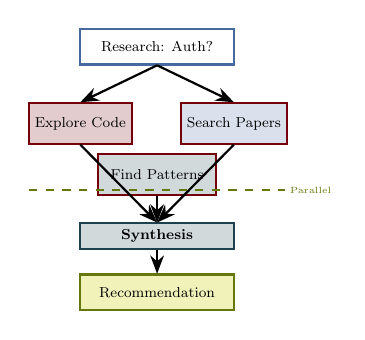
\begin{tikzpicture}[scale=0.65, transform shape]
                % Research task
                \node[processbox,minimum width=3cm] (task) at (1.5,4) {Research: Auth?};

                % Three parallel agents
                \node[agentbox,fill=UofSCGarnet!20,minimum width=2cm] (a1) at (0,2.5) {Explore Code};
                \node[agentbox,fill=UofSCAtlantic!20,minimum width=2cm] (a2) at (3,2.5) {Search Papers};
                \node[agentbox,fill=UofSCCongaree!20,minimum width=2.3cm] (a3) at (1.5,1.5) {Find Patterns};

                % Sync
                \node[syncbox,minimum width=3cm] (sync) at (1.5,0.3) {Synthesis};

                % Result
                \node[resultbox,minimum width=3cm] (result) at (1.5,-0.8) {Recommendation};

                % Arrows
                \draw[myarrow] (task.south) -- (a1.north);
                \draw[myarrow] (task.south) -- (a2.north);
                \draw[myarrow] (a1.south) -- (sync.north);
                \draw[myarrow] (a2.south) -- (sync.north);
                \draw[myarrow] (a3.south) -- (sync.north);
                \draw[myarrow] (sync.south) -- (result.north);

                % Parallel indicator
                \draw[thick,UofSCHorseshoe,dashed] (-1,1.2) -- (4,1.2);
                \node[font=\tiny,UofSCHorseshoe] at (4.5,1.2) {Parallel};
            \end{tikzpicture}
\end{document}
